\section{Theory of Operations}

\subsection{I2C Core Features}
\begin{itemize}
    \item \textbf{Two-Wire Interface:} SDA (data) + SCL (clock).
    \item \textbf{Configurable Speeds:} Standard (100\,kHz), Fast (400\,kHz), Fast+ (1\,MHz).
    \item \textbf{Master or Slave Mode:} Switch via control registers or synthesis parameters.
    \item \textbf{Hardware Arbitration:} For multi-master bus conflicts.
    \item \textbf{Address Recognition:} 7-bit or masked addresses, optional secondary address.
    \item \textbf{Smart Mode (Auto ACK):} Simplifies software overhead during high-speed data transfers.
    \item \textbf{SMBus Compatibility:} Includes time-out detection, Quick Command, etc.
\end{itemize}

\subsection{Block Diagram}
\begin{figure}[H]
    \centering
    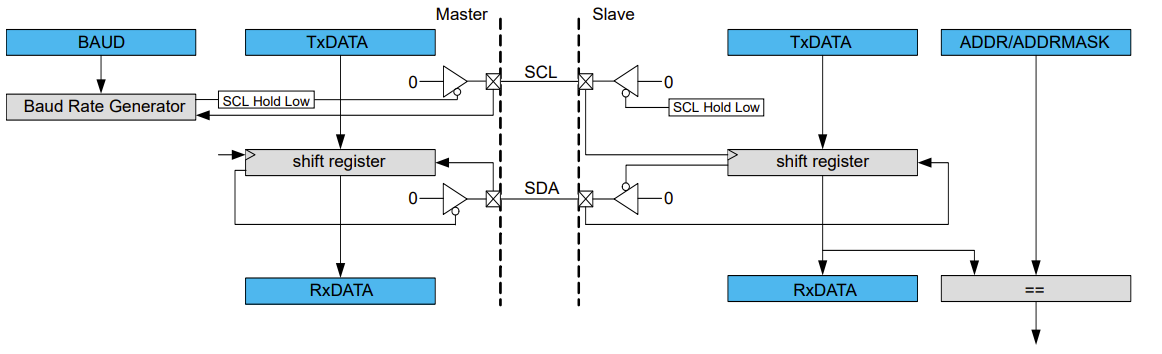
\includegraphics[width=0.75\textwidth]{images/i2c_block_diagram.png} % Replace with your actual figure
    \caption{I2C Core Block Diagram (Example)}
    \label{fig:i2c_block_diagram}
\end{figure}

\subsection{Overview}
The I2C protocol is well-suited for on-board communication where multiple ICs need addressing and simple read/write operations. The block diagram above shows a typical architecture with separate Master and Slave sub-blocks, optional Dual Mode logic, and registers to control and monitor the bus state.

\subsection{Typical Use Cases}
\begin{itemize}
    \item \textbf{Sensor Interfacing:} Reading/writing registers in sensor devices (temperature, pressure, etc.).
    \item \textbf{EEPROM/FRAM Storage:} Storing configuration or calibration data.
    \item \textbf{Multi-MCU Communication:} Simple messaging between multiple microcontrollers.
    \item \textbf{SMBus Power Components:} Controlling power regulators, battery chargers, etc.
\end{itemize}
